\subsection{Impact of misjudging the selection function of the data set} \label{sec:results_incompR}

The SF (see Section \ref{sec:selectionfunction}) can be very complex and is therefore sometimes not perfectly known. Here we investigate how much this could affect the recovery of the potential. We do this by creating mock data in a spherical survey volume around the Sun (see Test \ref{test:isoSphFlexIncomp} in Table \ref{tbl:tests}) and a spatially varying completeness function
\begin{equation}
\text{completeness}(r) \equiv 1- \epsilon_r \frac{r}{r_\text{max}}, \label{eq:rad_incomp}
\end{equation}
which drops linearly with distance $r$ from the Sun. In the \RM{} analysis however, we assume constant completeness ($\epsilon_r=0$). The incompleteness parameter $\epsilon_r$ of the mock data quantifies therefore by how much we misjudge the SF. This captures the relevant case of stars being less likely to be observed (than assumed) the further away they are (e.g., due to unknown dust obscuration). 

%==================================================

%FIGURE: isoSphFlexIncompR

\begin{figure}[!htbp]
\centering
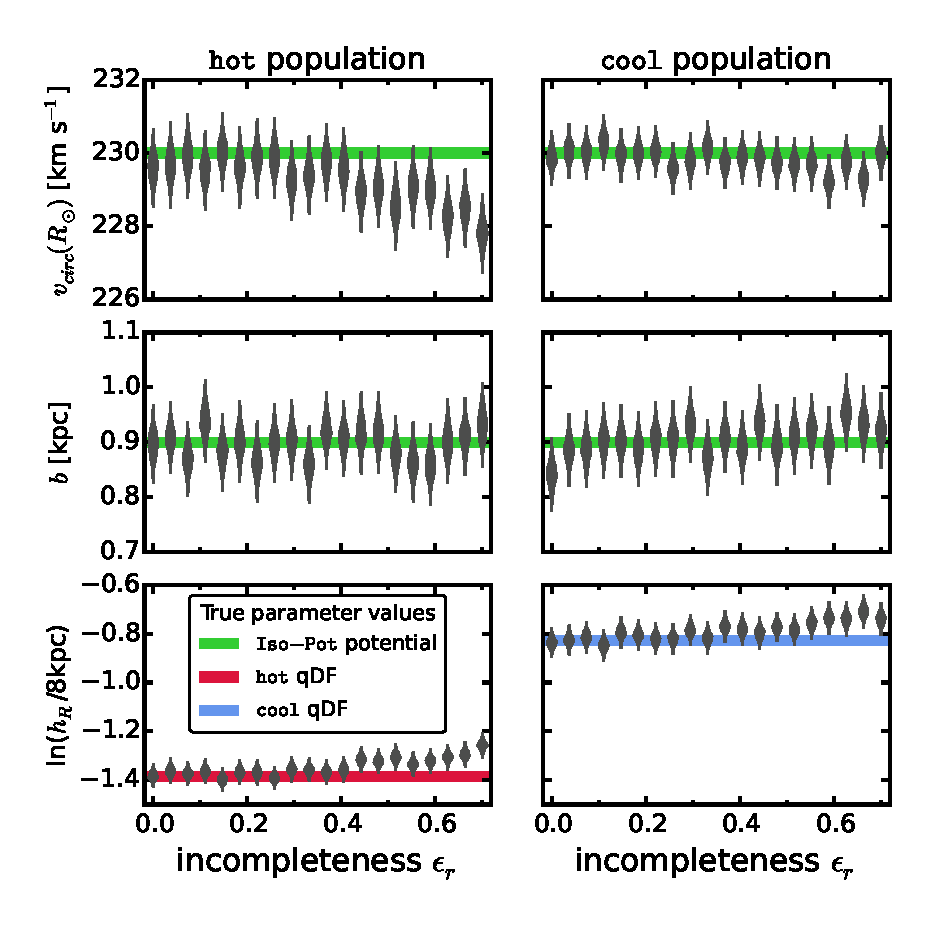
\includegraphics[width=\columnwidth]{figs/isoSphFlexIncompR_violins_2.eps}
\caption{Impact of misjudging the radial completeness of the data on the parameter recovery with \RM{}. Each mock data set was created with a different incompleteness parameter $\epsilon_r$ (shown on the $x$-axis, see Equation \ref{eq:rad_incomp}). (The model parameters are given as Test \ref{test:isoSphFlexIncomp} in Table \ref{tbl:tests}.) The analysis however did not know about the incompleteness and assumed that all data sets had constant completeness within the survey volume ($\epsilon_r = 0$). The violins show the full shape of the projected \pdf{}s for each model parameter, and the solid lines their true values. The \RM{} method seems to be very robust against small to intermediate deviations between the true and the assumed data incompleteness. (The qDF parameters not shown here exhibit a similar robustness as $h_R$.)} 
\label{fig:isoSphFlexIncompR_violins}
\end{figure}

\begin{figure}[!htbp]
\centering
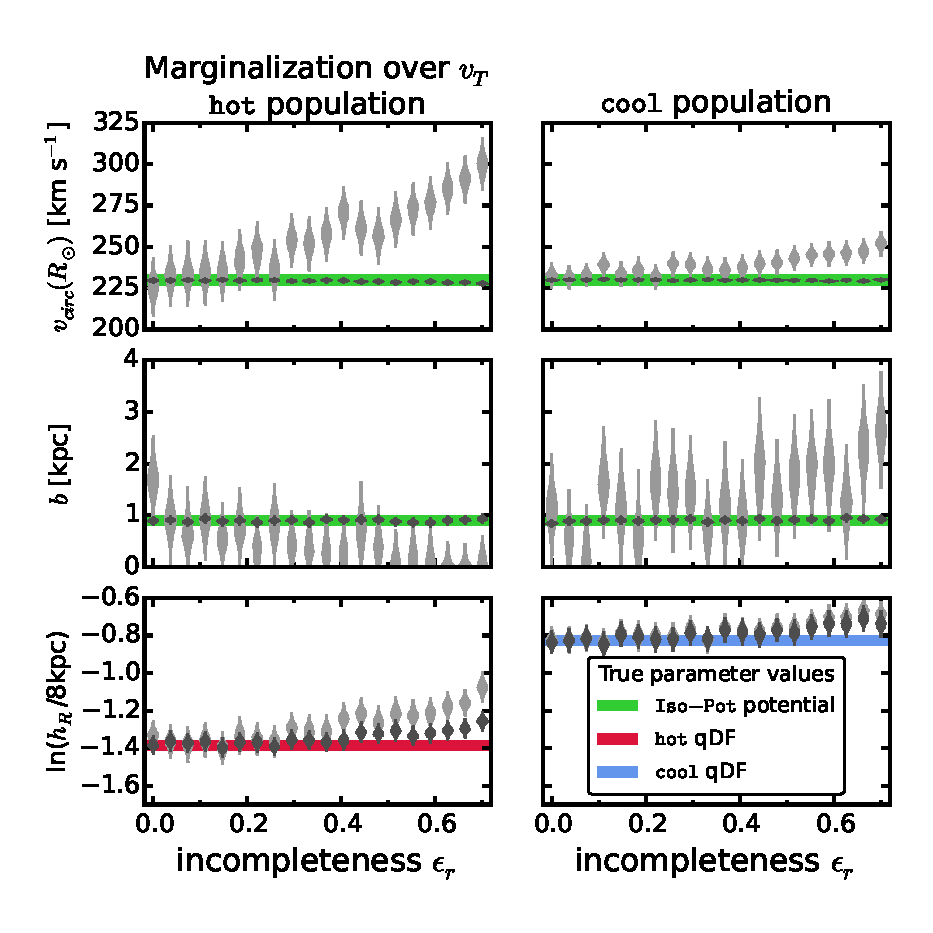
\includegraphics[width=\columnwidth]{figs/isoSphFlexIncompR_marginal_violins_3.eps}
\caption{Same as Figure \ref{fig:isoSphFlexIncompR_violins}, but without including information about the tangential velocities in the analysis. This was done by marginalizing the likelihood in Equation \ref{eq:prob} over $v_T$ (bright grey violins; the dark grey violins are the same as in Figure \ref{fig:isoSphFlexIncompR_violins} for comparison). The parameter recovery is much worse than in Figure \ref{fig:isoSphFlexIncompR_violins}. This could indicate that much of the information about the potential is actually stored in the rotation curve, i.e., $v_T(R)$, which is not affected by removing stars from the data set. But even if we do not include $v_T$ we can still recover the potential within the errors, at least for small ($\epsilon_r \lesssim 0.15$).} 
\label{fig:isoSphFlexIncompR_marginal_violins}
\end{figure}

%==================================================

Figure \ref{fig:isoSphFlexIncompR_violins} demonstrates that the potential recovery with \RM{} is very robust against somewhat wrong assumptions about the radial completeness of the data. The robustness for the \texttt{cool} stellar population is even more striking than for the \texttt{hot} population. The reason for this robustness could be, that much information about the potential comes from the rotation curve measurements in the plane, which is not affected by the incompleteness of the sample. We test this by analysing the data sets from Figure \ref{fig:isoSphFlexIncompR_violins} again, but this time not including tangential velocity measurements (which is done by marginalizing the likelihood in Equation \ref{eq:prob} over $v_T$). Figure \ref{fig:isoSphFlexIncompR_marginal_violins} shows that in this case the potential is much less tightly constrained, even for 20,000 stars. For only small deviations of true and assumed completeness ($\epsilon_r \lesssim 0.15$) the true potential is however still included within the errors of our fitting result (see Figure \ref{fig:isoSphFlexIncompR_marginal_violins}).

We found similarly robust results also for a misjudgement of spatial completeness functions varying with the distance from the plane, $|z|$.


%=============================